%! TEX root = ./master.tex

\lecture{11}{Week 6}{}

\subsubsection{\code{switch} statement}
We could implement a switch as a bunch of \code{if then else} and \code{goto} but that gets complicated with fall through and there would be very many comparisons. So compilers do not to that. Firstly, they differentiate between dense and spares \code{swtich} statements. 

\paragraph{Dense \code{switch}}
In a dense \code{switch} the values of \code{x} lie close together. For each possible case block the compiler creates an entry in the jump table. This includes cases, which land at the default. We can regard the jump table as an array which gives us for a given \code{x} the address to the jump target, which we want to execute in this case.

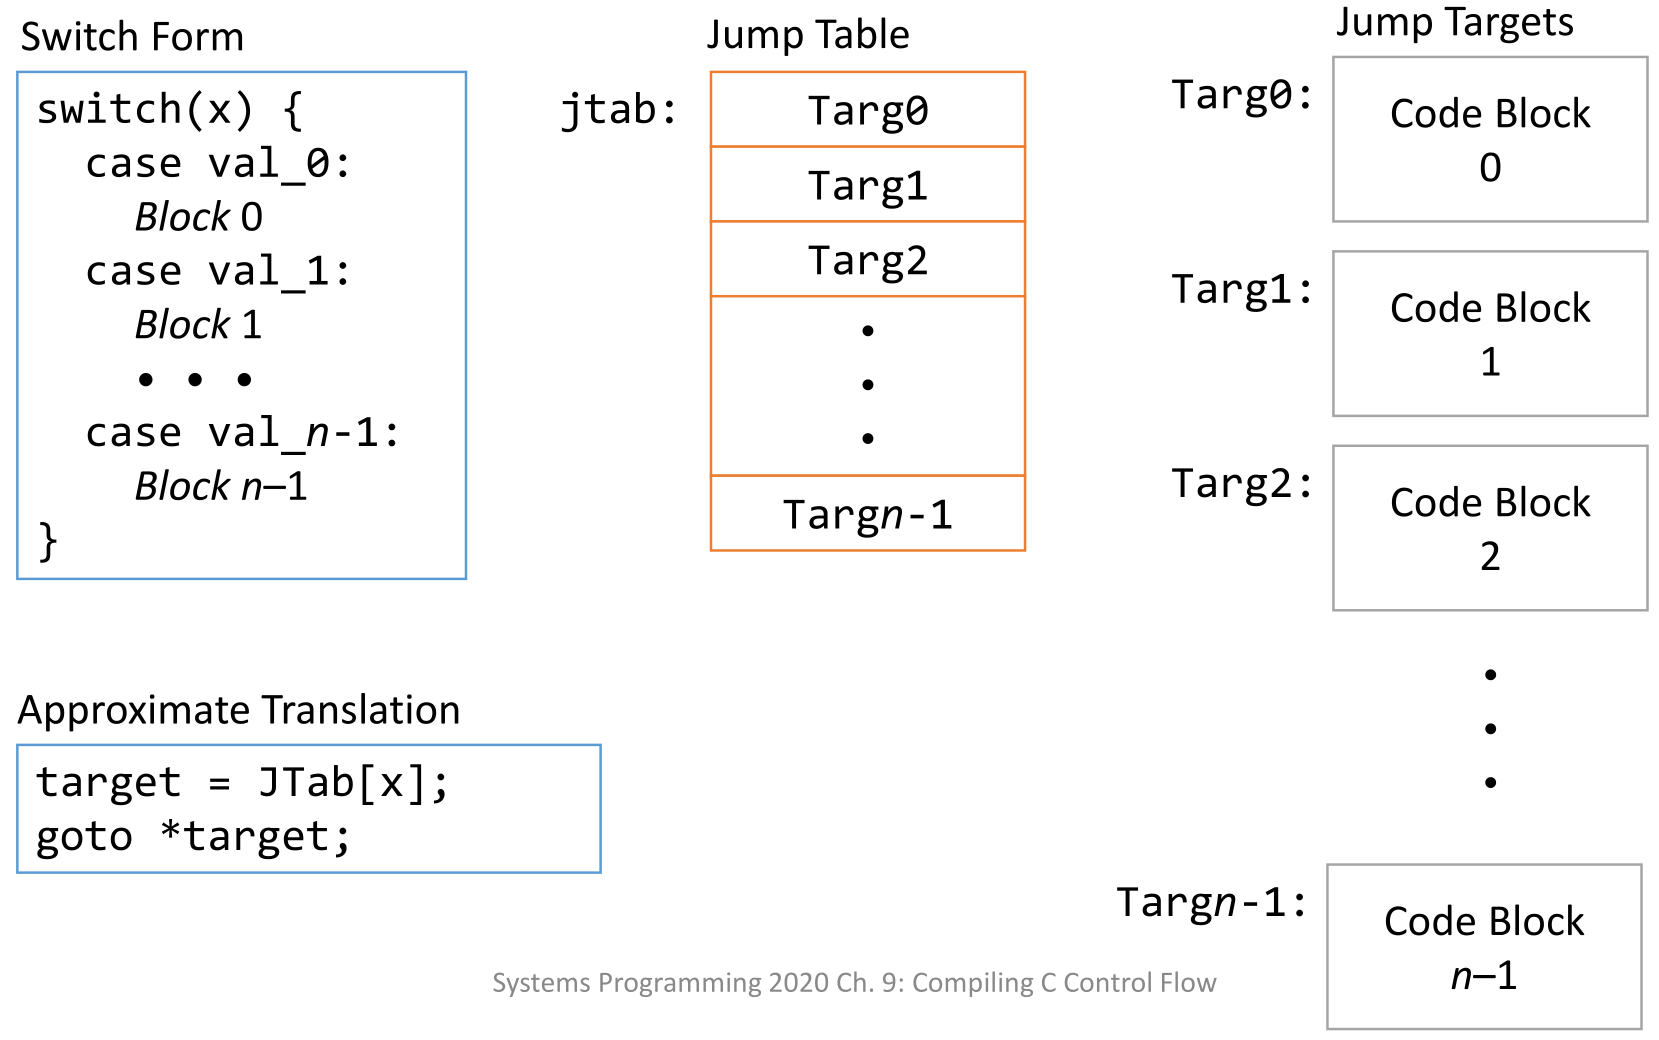
\includegraphics[width=0.8\textwidth]{11_denseswitchOverview.png}

The usage of the jump table makes the actual switch statement extremely compact. It actually only consists of a comparison, a conditional jump to the default block, and a indirect jump, via the jump table, to the designated jump target. This indirect jump could be implemented as \code{jmp *.L4(,\%rdi, 8)}, where \code{.L4} is the base address and \code{\%rdi} holds our \code{x}. We scale by $8$ since labels are $64$ bit on x86-64.

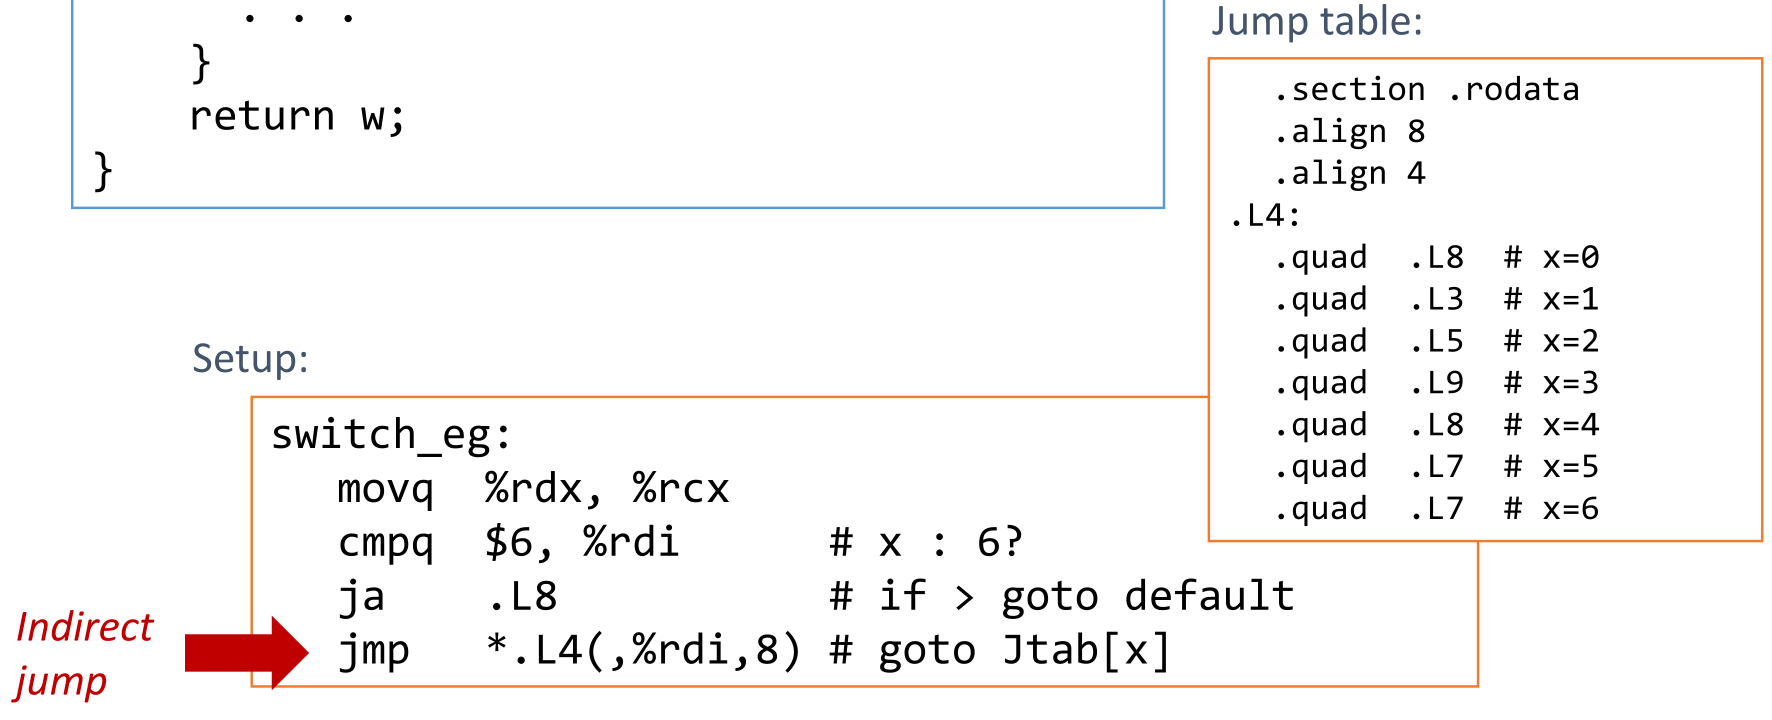
\includegraphics[width=0.8\textwidth]{11_denseswitchsetup.png}

The jump table does not seem to be in an order, that is because the compiler orders in in a way that it is most efficient.

Jump table is just data, so it does not show up in assembly or disassembled code. Nevertheless, we can inspect it using \code{gdb}.

\paragraph{Spare \code{switch}}
When there are many cases which should result in the default action, it is often too expensive to create a jump table for all these default entries. In these cases, compiler do create an binary three with three actions per node. A less than, equal and greater than. This yields logarithmic performance. In assembly this is achieved by a series of conditional jumps.

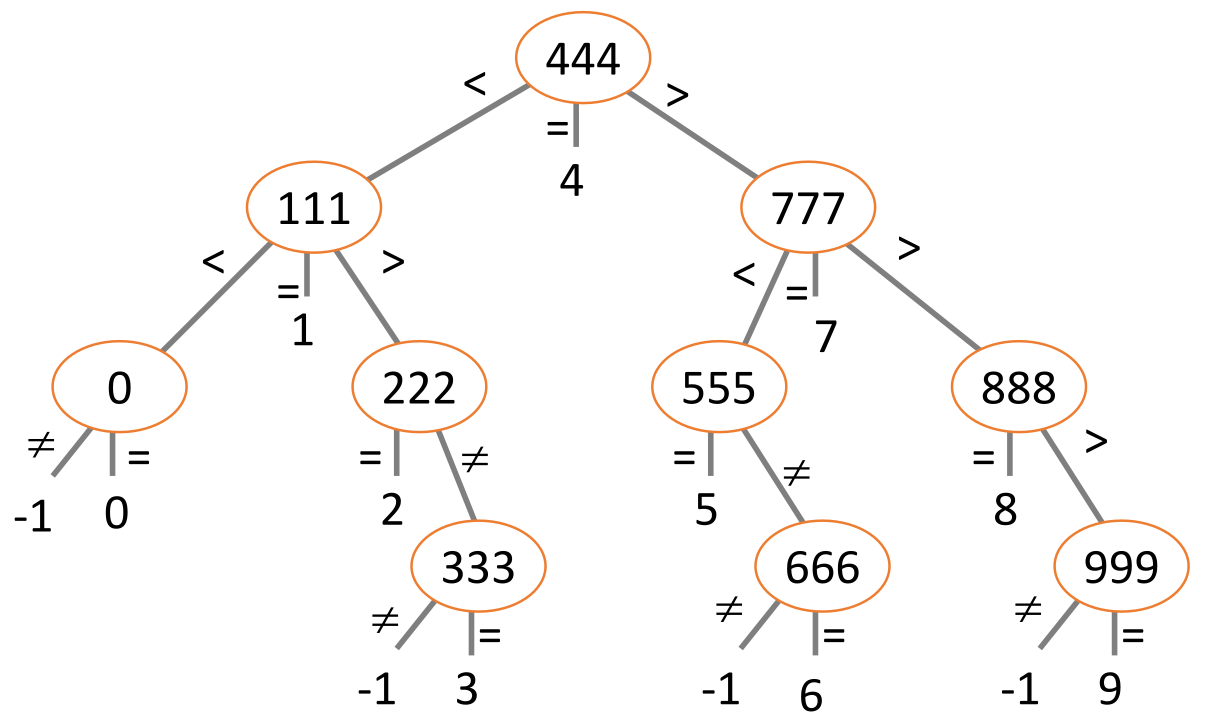
\includegraphics[width=0.8\textwidth]{11_sparseswitchtree.png}

The compile are very smart about when to use a jump table and then to rely on a search tree. We should trust the compiler in choosing the most suitable type. They may even create combinations of both types.

\subsubsection{Procedure Calls and Return}
\paragraph{Stack}
The stack is in our memory space. It starts at the top and grows downwards to lower adressess. \code{\%rsp} is the stack pointer which always points to the top (lowest address) of the stack. The stack provides the following typical CISC instructions:

\begin{description}
    \item[\code{pushl Src}:] Fetches the operand at \code{Src}, decrements the stack pointer by $4$ and writes the operand at to \code{\%rsp}.
    \item[\code{popl Dest}:] Reads the operand at the address pointed to by \code{\%rsp}, increments the stack pointer by $4$ and writes the operand to \code{Dest}.
\end{description}

These two operations are not that often used on x86-64. Even though they are very slim instructions, they are often replaced by other read and writes to relative addresses of the stack pointer.

\paragraph{Procedure Control Flow}
The stack is vital for procedure calls and returns. It is used to hold arguments, return values as well as return addresses.

In order to call a procedure, we call \code{call label}. This instruction pushed the return address on the stack and then jumps to \code{label}. The return address it vital in order to get back to the right place after the procedure has finished. In order to prevent the procedure to be called again after returning, the return address has to actually point on the address following the call instruction.

The instruction \code{ret} is called from a procedure. It pops the return address from the stack and jumps to this address.

There is no need to return after a call. This is in essence simple jump. RISC systems save the return address in a register and do not use a stack. This is called a \textit{wheeler jump}.

\paragraph{Stack Frame}
The stack frame is the current status of the stack. Generally speaking, it has the following structure.

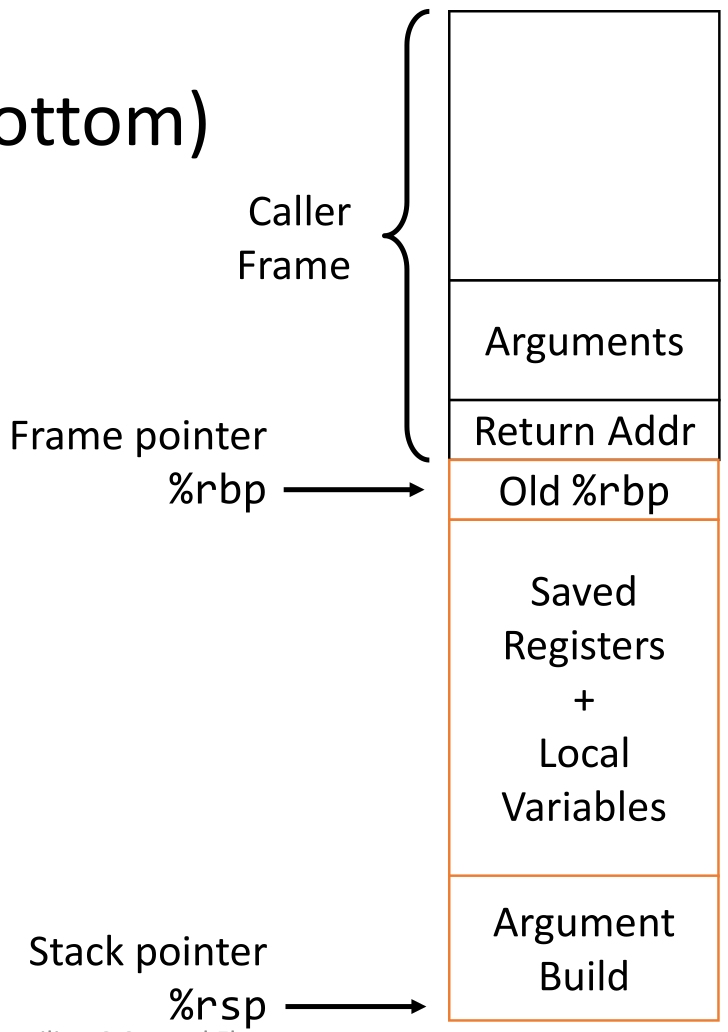
\includegraphics[width=0.4\textwidth]{11_stackframe.png}

The \textit{current stack} is the part between stack pointer and the \textit{frame pointer} \code{\%rbp}. The frame pointer points to the start of the current frame (frame contains everything related to the current procedure). At the top there are the \textit{Argument build}. It is actually not that often used nowadays. There we prepare the arguments for the function we are going to call. On top of that, there are the \textit{local variables}, which is data which we cannot keep in a register as well as the saved register content. And at the top of the current stack frame, appointed by the frame pointer, there is the \code{\%rbp} stored, of the previous frame.

Above, we find the caller's stack frame. It contains the return address and arguments passed to the call of the current procedure.

\subsubsection{Calling Convection}
There are certain conventions to which one should stick when calling procedures, and working with registers and the stack.

How do you construction procedure calls using these utilities.

\paragraph{Register Saving Conventions}
When one procedure calls another, then the one which initiates the calls ins the \textit{caller} and the one being called is the \textit{callee}. It has to be defined, which register who may change one which should stay untouched. There are the following two register types:

\begin{description}
    \item[Caller Saved:] These registers may be overwritten by the callee and therefore, it is the caller's responsibility to save them to their stack in case it needs them after the procedure returns.
    \item[Callee Saved:] These registers are long-lived and should not be overwritten by the callee. Hence, when using them they have to restore then before returning.
\end{description}

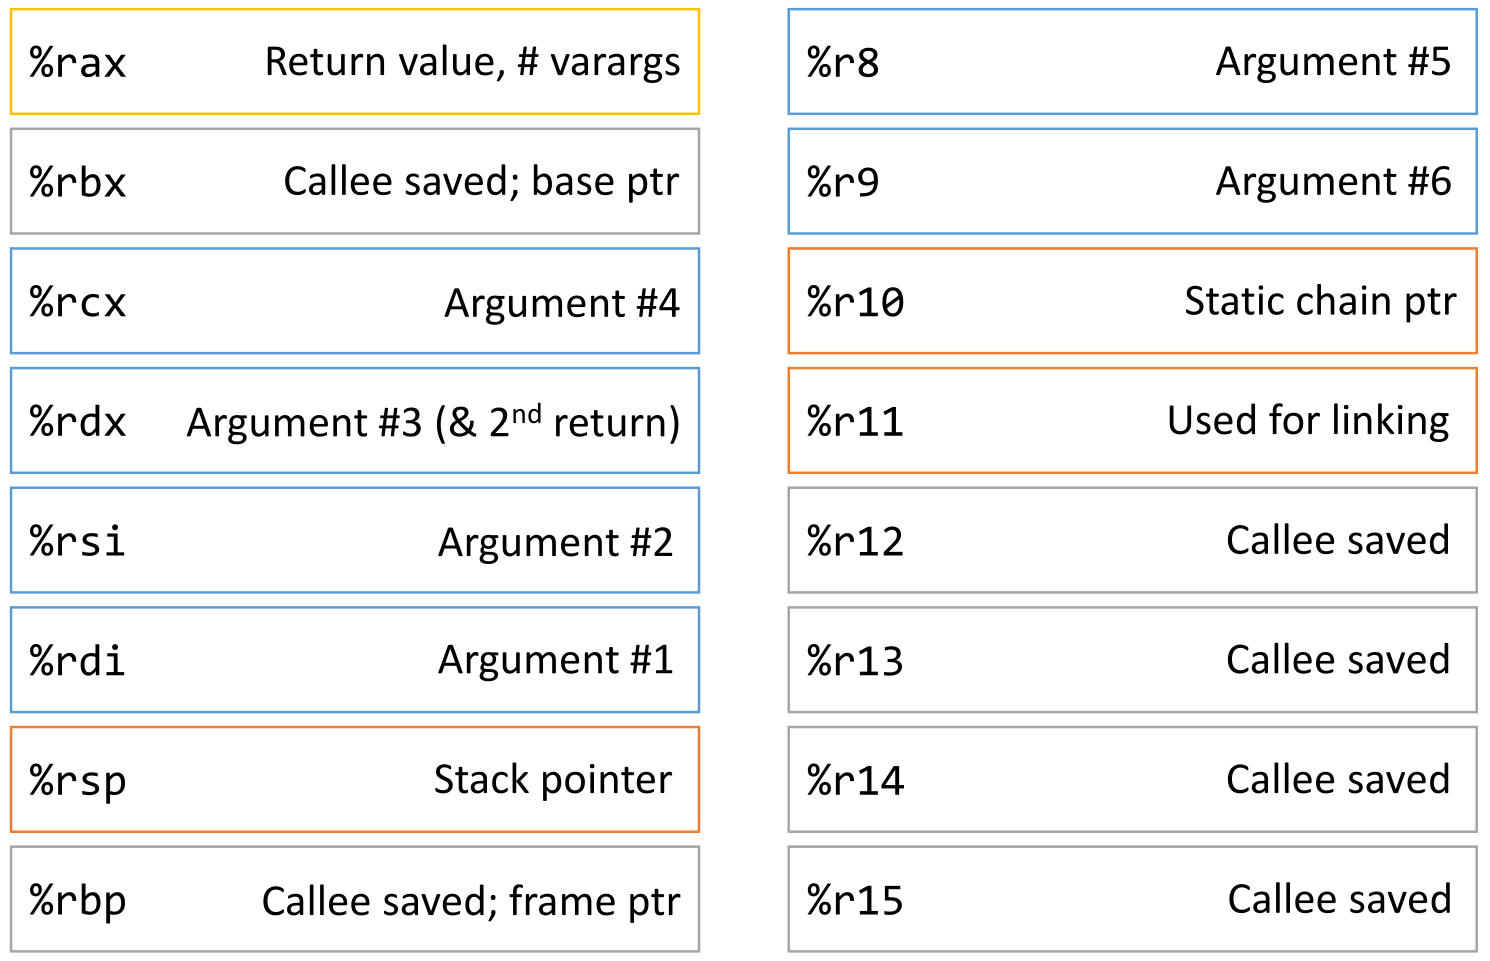
\includegraphics[width=0.8\textwidth]{11_registeroverview.png}

Arguments are passed to the callee via registers. If more than $6$ arguments are passed, the rest is passed via the stack. These registers are also used used as caller-saved and hence, can be altered by the callee.

There are two return registers. This way structs of size less than $128$ bits can be returned. If they exceed this size, they are put on the stack.

All in all, genreal purpose registers are not actually not really general purpose.

\paragraph{Working with the Stack and Stack Pointer}
All references to the stack are via the stack pointer. When the compiler adds several values to the stack (e.g. to restore callee-saved registers) it often adds then relative to the stack pointer, and decrements the stack pointer only after adding all elements. This is done for optimisation reason since the stack pointer is not decremented several times. The newly added values, which are not yet actually on the stack (stack pointer not yet updated) are in the so called \textit{red zone}.

Optimisation actions as such may break some conventions however, since it does not influence other parts, it is actually acceptable.

Other tricks are to not use the stack, to not use any callee-saved registers. In a \textit{tail call} we no not even push the current address to the stack when calling. This is useful when nested functions return (i.e. there is no need to return the inner function, just jump to the outer function which then returns). This prevents stack overflow for recursive function calls. All in all, often the stack frame is not very heavily used.
